\documentclass[11pt, oneside]{article}   	% use "amsart" instead of "article" for AMSLaTeX format
\usepackage[utf8]{inputenc}

\usepackage{lmodern}
\usepackage[T2A]{fontenc}
\usepackage{cmbright}
\usepackage[russian]{babel}
%\usetheme{Darmstadt}


\usepackage{amsmath}
\usepackage{amsfonts}
\usepackage{amssymb}
\usepackage{bm}
\usepackage{graphicx}
% Использовать полужирное начертание для векторов
\let\vec=\mathbf

\DeclareMathOperator{\mathspan}{span}
\DeclareMathOperator{\mathdim}{dim}
\DeclareMathOperator{\rank}{rank}
\DeclareMathOperator{\diag}{diag}

\begin{document}
	\author{Е. Ларин, Ф. Ежов, И. Кононыхин }
	\title{Обучение с учителем. Классификация. Дискриминантный анализ. }
%	\subtitle{Санкт-Петербургский государственный университет 
%		
%		Прикладная математика и информатика
%		
%		Вычислительная стохастика и статистические модели
%	}
	\date{}
	%\subject{Семинар по статистическому и машинному обучению}


		\maketitle 

		\section{Обучение с учителем}
		Рассмотрим задачу обучения с учителем, частным случаем которой являются задачи классификации и регрессии.

		Алгоритм в общем виде имеет вид:
		\begin{itemize}
			\item \textit{Вход}: $\bm{X}$ --- выборка $\bm{\xi}$, случайной величины признаков, $\bm{y}$ --- выборка $\eta$, случайной величны <<ответов>> (принадлежность к классу для классификации, либо значение функции для регрессии). Предполагаем, что существует неизвестное отображение $y^*: \bm{\xi} \to \eta$  (гипотеза непрерывности или компактности)
			
			\item \textit{Задача}: По $\bm{X}$ и $\bm{y}$ найти такое отображение $\hat{y}^*: \bm{\xi} \to \eta$, которое приблизит отображение  $y^*$. 
			
			\item \textit{Оценка}: Функция потерь $\mathfrak{L}(y^*(x), \hat{y}^*(x))$. Здесь $x$ --- реализация $\bm{\xi}$
		\end{itemize}
		
		\subsection{Отступы}
		\label{margins}
		Введем понятие отступов. Пусть 	$\Phi(\bm{x}, \beta) = sign  (g(\bm{x}, \beta))$ --- разделяющий классификатор. Тогда $g(\bm{x}, \beta)$ --- разделяющая функция, а $g(\bm{x}, \beta) = 0$ --- уравнение разделяющей поверхности. Отступом для объекта $x_i$ будем называть значение $M_i(\beta)$, такое что $M_i(\beta) = g(\bm{x}_i, \beta) y_i$. Если $M_i(\beta) < 0$, тогда алгоритм ошибается на $\bm{x}_i$, иначе алгоритм классифицировал объект верно. Чем больше значение $|M_i(\beta)|$, тем больше уверенность в правильности или неправильности классификации объекта.
		
		\section{Классификация}
		Перейдём к задаче классификации. Как и в задаче регрессии, данные должны происходить из некоторой генеральной совокупности. 
		
		Будем рассматривать выборку признаков и ответов~\ref{1}
		\begin{equation}
			\bm{X} \in \mathbb{R}^{n\times p}, \;\;\mathbf{y}\in \mathbb{A}^n.
			\label{1}
		\end{equation}
		
		Отметим, что множество $\mathbb{A}^n$ не является непрерывным. Размерность этого множества $k\times n$, где $k$ --- количество возможных классов.
		
		Для обоснования применения методов классификации используется \textbf{\textit{гипотеза компактности}}:
		
		<<Близкие>> объекты, как правило, принадлежат одному классу.
		\newline



		\subsection{Классификация: вероятностная постановка}
		Поставим задачу классификации в терминах генеральных случайный величин.
		
		\textit{Дано:}
		\begin{itemize}
			\item $\bm{\xi} \in \mathbb{R}^p$ --- вектор признаков
			\item $\eta \in \mathbb{A}$ --- классовая принадлежность
		\end{itemize}
	
		Предположение об их зависимости можно записать в виде \ref{2}.
		\begin{equation}
			\eta = \Phi(\bm{\xi})
			\label{2}
		\end{equation}
		
		\textit{Задача:} найти $\Phi$
		
		При переходе к выборкам, случайная величина признаков $\bm{\xi}$ заменяется на матрицу наблюдений $\bm{X}$, а случайная величина ответов $\eta$ --- на вектор классовой принадлежности $\bm{y}$.
		
		Предположение принимает вид \ref{3}.
		\begin{equation}
			y_i = \Phi(\bm{x}_i),\;\;\; i = 1, \ldots, n
			\label{3}
		\end{equation}
		

		\subsection{Классификация: оценка качества}
		\label{metrics}
		\begin{figure}
			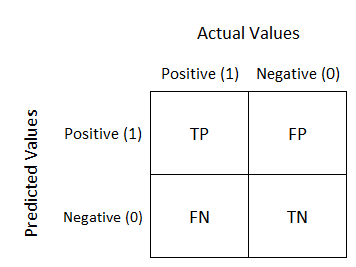
\includegraphics[width=0.7\linewidth]{imgs/conf_matrix}
			\label{conf_matrix}
			
		\end{figure}
	    На основе матрицы ошибок~\ref{conf_matrix} есть большое количество разных метрик. Приведём некоторые из них: 
	    \begin{itemize}
	    	\item\textit{accuracy} = ${TP + TN}\over{TP+TN+FP+FN}$, 
	    	\item\textit{recall} = ${TP}\over{TP+FN}$, 
	    	\item\textit{precision} = ${TP}\over{TP+FP}$, 
	    	\item $F_\beta = (1-\beta^2) {{precision \times recall}\over{(\beta^2 \times precision) + recall}}$, 
	    	\item\textit{ROC--AUC}
	    \end{itemize}


		\subsection{Классификация: этапы обучения модели}
		\begin{itemize}
			\item Выбор модели (класс рассматриваемых $\Phi$ из \ref{3}).
					 Здесь будут рассмотрены модели LDA и QDA. 
			\item Выбор функции потерь.
					 Чаще всего это $\sum_{i=1}^{n}(y_i \neq \widehat{y}_i)$.
			\item Выбор метода обучения.
			 		Выбор способа подбора параметров для минимизации функции потерь на обучающем множестве.
			\item Выбор метода проверки.
			 		Выбор оценки качества модели, например, с помощью метрик из раздела~\ref{metrics}.
		\end{itemize}

%		\subsection{Классификация: задача оптимизации}
%		\begin{itemize}
%			\item $\hat{\beta}$ --- параметры модели
%			\item $\bm{\Phi}(\bm{x}, \beta)$ --- функционал классификации
%			\item $\mathfrak{L}(\bm{\Phi}(\bm{x}, \beta), \bm{y})$ --- функция потерь (метрика)
%		\end{itemize}
%		\begin{block}{}
%			$$\hat{\beta} = \arg\min_{\beta} \mathfrak{L}(\bm{\Phi}(\bm{x}, \beta), \bm{y})$$
%		\end{block}

		\subsection{Классификация: общий подход к решению}
		Как построить функционал $\Phi$?
		
		
		Общий подход --- построить набор классифицирующих функций $f_i$, $i = 1, \ldots, K$. Каждая функция $f_i(\bm{x})$ показывает меру принадлежности $\bm{x}$ классу $i$. 
		
		Таким образом, решение о принадлежности классу принимается при обнаружении классифицирующей функции с наибольшим значением:
		\begin{equation}
			\Phi(\bm{x}) = \arg\max_i(f_i(\bm{x})).
			\label{4}
		\end{equation}

		\section{Дискриминантный анализ}
		Примем за функции $f_i$ из \ref{4} оценку вероятности принадлежности к $i$-му классу.
		
		$$\Phi(\bm{x}) = \arg\max_i (P(C_i|\bm{x})).$$
		
		$C_i$ ---  класс, состоящий из одного события: $\bm{x}$ принадлежит $i$-му классу.

		Если известны априорные вероятности получения $i$-го класса ($\pi_i$), применим формулу Байеса
		
		$$P(C_i|\bm{x}) = {{\pi_i P(\bm{x}|C_i)}\over{\sum_{j=1}^{K} \pi_j P(\bm{x}|C_j)}}.$$
		 
		 Отбросим знаменатель
		
		$$f_i = P(C_i|\bm{x}) = \pi_i P(\bm{x}|C_i).$$
 
		\subsection{LDA}
		Предположим, что искомые классы имеют многомерное нормальное распределение с равными дисперсиями.
		
		Запишем это в виде формулы:

		$$\mathtt{P}(\bm{\xi}|\eta = A_i) = \mathtt{N}(\bm{\mu}_i, \bm{\Sigma})$$
		
		Построим классифицирующие функции:
		$$f_i(\bm{x}) = {{\pi_i}\over{(2\pi)^{p/2}|\bm{\Sigma}|^{1/2}}}exp\left(-{{1}\over{2}}(\bm{x} - \bm{\mu}_i)\bm{\Sigma}^{-1}(\bm{x} - \bm{\mu}_i)^\mathtt{T}\right)$$
		
		Немного упростим (подробнее было изложено в одном из предыдущих курсов):
		\begin{equation}
			h_i(\bm{x}) = -0.5 \bm{\mu}_i\bm{\Sigma}^{-1}\bm{\mu}_i^\mathtt{T} + \bm{\mu}_i\bm{\Sigma}^{-1}\bm{x} + \log\pi_i
		\label{lda}
		\end{equation}
		Функции~\ref{lda} применяются при классификации данным методом.


		\subsection{QDA}
		
		Предположим, что искомые классы имеют многомерное нормальное распределение с различными дисперсиями.
		
		Запишем это в виде формулы:
		$$\mathtt{P}(\bm{\xi}|\eta = A_i) = \mathtt{N}(\bm{\mu}_i, \bm{\Sigma}_i)$$
		
		Построим классифицирующие функции:
		$$f_i(\bm{x}) = {{\pi_i}\over{(2\pi)^{p/2}|\bm{\Sigma}_i|^{1/2}}}exp\left(-{{1}\over{2}}(\bm{x} - \bm{\mu}_i)\bm{\Sigma}_i^{-1}(\bm{x} - \bm{\mu}_i)^\mathtt{T}\right)$$
		
		Немного упростим (подробнее было изложено в одном из предыдущих курсов):
		\begin{equation}
			g_i(\bm{x}) = -0.5 (\bm{x} - \bm{\mu}_i)\bm{\Sigma}^{-1}(\bm{x} - \bm{\mu}_i)^\mathtt{T} - 0.5\log|\bm{\Sigma}_i| + \log\pi_i
			\label{qda}
		\end{equation}
		
		Функции~\ref{qda} применяются при классификации данным методом.

%		\section{Классификация и регрессия}
%		
%		Сравним модели линейной регрессии и бинарной классификации.
%		\subsection{Регрессия}
%		Обучающая выборка: $\bm{X} \in \mathbb{R}^{n \times p}, \;\;\mathbf{y}\in \mathbb{R}^n$.
%		
%		\begin{enumerate}
%			\item Модель регрессии:
%			$$ \hat{\bm{y}} = \bm{\Phi}(\bm{x}, \beta) = \langle \bm{x}, \beta \rangle = \sum\limits_{j=1}^{p} \beta_j x_j , \; \beta \in \mathbb{R}^p$$
%			
%			\item Функция потерь:
%			$$ \mathfrak{L}(\hat{\bm{y}}, \bm{y}) = (\hat{\bm{y}} - \bm{y})^2$$
%			
%			
%			\item Метод обучения --- метод наименьших квадратов:
%			$$ Q(\beta) = \sum\limits_{i = 1}^{n} (\bm{\Phi}(\bm{x}_i, \beta) - \bm{y}_i)^2 \rightarrow \min\limits_{\beta} $$
%			
%		\end{enumerate}
%
%		\subsection{Классификация}
%		Обучающая выборка: $\bm{X} \in \mathbb{R}^{n\times p}, \;\; y \in \{-1, 1\}$.
%		
%		\begin{enumerate}
%			\item Модель классификации:
%			$$ \hat{y} = \bm{\Phi}(\bm{x}, \beta) = sign \langle \bm{x}, \beta \rangle = sign \sum\limits_{j=1}^{p} \beta_j x_j , \; \beta \in \mathbb{R}^p$$
%			
%			\item Функция потерь:
%			$$ \mathfrak{L}(\hat{y}, y) = [\hat{y} y < 0] = [ \langle \bm{x}, \beta \rangle y < 0 ] \leq \hat{\mathfrak{L}}( \langle \bm{x}, \beta \rangle y) $$
%			
%			
%			\item Метод обучения --- минимизация эмпирического риска:
%			$$ Q(\beta) = \sum\limits_{i = 1}^{n} [\langle \bm{x}_i, \beta \rangle y_i < 0] \leq \sum\limits_{i = 1}^{n} \hat{\mathfrak{L}}( \langle \bm{x}_i, \beta \rangle y_i)  \rightarrow \min\limits_{\beta} $$
%			
%		\end{enumerate}
%
%		\section{Отступы}
%		
%		$\bm{\Phi}(\bm{x}, \beta) = sign  (g(\bm{x}, \beta))$ --- разделяющий классификатор,\\
%		$g(\bm{x}, \beta)$ --- разделяющая функция,\\
%		$g(\bm{x}, \beta) = 0$ --- уравнение разделяющей поверхности.\\
%		
%		\bigskip
%		
%		$M_i(\beta) = g(\bm{x}_i, \beta) y_i$ --- отступ объекта $\bm{x}_i$. \\
%		Если $M_i(\beta) < 0$, тогда алгоритм ошибается на $\bm{x}_i$.
%	
%
%		\section{Отступы}
%		\begin{figure}
%			\centering
%			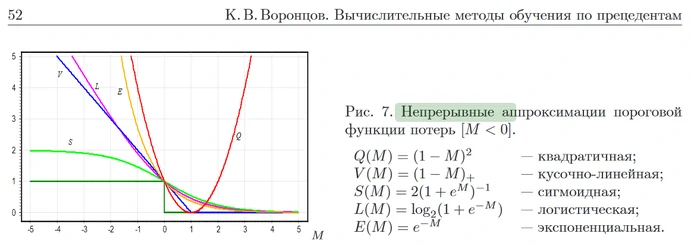
\includegraphics[width=0.7\linewidth]{imgs/margins}
%			
%
%		\end{figure}

\section{Логистическая регрессия}

Дана выборка $\bm{X} \in \mathbb{R}^{n\times p}$. Поставим задачу классификации объектов $\bm{x}_i$ на два класса $\{-1, 1\}$. 

\subsection{Подход через минимизацию функции потерь}

Воспользуемся линейной моделью для решение задачи классификации:

\begin{equation}
	\hat{y} = \Phi(\bm{x}, \beta) = sign \langle \bm{x}, \beta \rangle
	\label{7}
\end{equation}

Функция потерь в данном случае будет:

\begin{equation}
	\mathfrak{L}(\hat{y}, y) = [\hat{y} y < 0] = [ \langle \bm{x}, \beta \rangle y < 0 ]
	\label{8}
\end{equation}

Задача минимизация записывается следующим образом:

\begin{equation}
	Q(\beta) = \sum\limits_{i = 1}^{n} [\langle \bm{x}_i, \beta \rangle y_i < 0] \rightarrow \min\limits_{\beta}
	\label{9}
\end{equation}

Перейдем от задачи \ref{9} к другой, заменив в \ref{8} функцию потерь на другую  ($ \hat{\mathfrak{L}} $) мажорирующую ее, получим:

\begin{equation}
	\mathfrak{L}(\hat{y}, y) = [ \langle \bm{x}, \beta \rangle y < 0 ] \leqslant \hat{\mathfrak{L}}( \langle \bm{x}, \beta \rangle y)
	\label{10}
\end{equation}

\begin{equation}
Q(\beta) = \sum\limits_{i = 1}^{n} [\langle \bm{x}_i, \beta \rangle y_i < 0] \leqslant \sum\limits_{i = 1}^{n} \hat{\mathfrak{L}}( \langle \bm{x}_i, \beta \rangle y_i)  \rightarrow \min\limits_{\beta}
\label{11}
\end{equation}

Видно, что аргумент функции потерь $\hat{\mathfrak{L}}$, это ничто иное как отступ $M_i$ для объекта в $\bm{x}_i$ введенный в главе \ref{margins}.

Чтобы линейная модель в задаче \ref{11} стала логистической регрессией, достаточно взять функцию потерь $\hat{\mathfrak{L}}(M_i) = \log(1 + e^{-M_i})$. Такая функция потерь называется логарифмической или логистической. 

Тогда задача минимизации \ref{11} запишется так:

\begin{equation}
	Q(\beta) = \sum\limits_{i = 1}^{n} \log(1 + e^{- \langle \bm{x}_i, \beta \rangle y_i})  \rightarrow \min\limits_{\beta}
	\label{12}
\end{equation}

Методы решение задачи минимизации:

\begin{itemize}
	\item метод стохастического градиента
	\item метод Ньютона-Рафсона
\end{itemize}

\subsection{Вероятностный подход}

Пусть $\sigma$ --- сигмоида и:

\begin{itemize}
	\item $P(y_i = 1 | \bm{x}_i; \beta) = \sigma_\beta(M_i) $, вероятность объекта $\bm{x}_i$ принадлежать классу $1$.
	\item $P(y_i = -1 | \bm{x}_i; \beta) = 1 - \sigma_\beta(M_i) $, вероятность объекта $\bm{x}_i$ принадлежать классу $-1$.
\end{itemize}

Тогда $P(y_i | \bm{x}_i; \beta) = \sigma_\beta(M) = \dfrac{1}{1 + e^{- \langle \bm{x}, \beta \rangle y}}$

Запишем логарифм функции правдоподобия:

\begin{equation}
	Q(\bm{X}, \beta) = \log \bm{L}(\beta) = \log 	
	\prod\limits_{i = 1}^{n} P(y_i | \bm{x}_i; \beta) = - \sum\limits_{i = 1}^{n} \log(1 + e^{- \langle \bm{x}_i, \beta \rangle y_i}) \rightarrow \max\limits_{\beta}
	\label{13}
\end{equation}

Заметим, что задача \ref{13} совпадает с задачей \ref{12}.

\subsection{Регуляризация}

В задачу минимизации можно добавить параметры $\beta$, тогда мы получим регуляризацию:

\begin{itemize}
	\item \textbf{L1 регуляризация:}  $$Q(\beta) = \sum\limits_{i = 1}^{n} \log(1 + e^{- \langle \bm{x}_i, \beta \rangle y_i}) + \lambda \sum\limits_{j = 1}^{p}|\beta_j| \rightarrow \min\limits_{\beta}$$
	\item \textbf{L2 регуляризация:}  $$Q(\beta) = \sum\limits_{i = 1}^{n} \log(1 + e^{- \langle \bm{x}_i, \beta \rangle y_i}) + \frac{\lambda}{2} \sum\limits_{j = 1}^{p}\beta_j^2 \rightarrow \min\limits_{\beta}$$
\end{itemize}

Параметр $\lambda$ отвечает за <<силу>> регуляризации и может быть подобран с помощью кросс-валидации.

\subsection{Многоклассовая логистическая регрессия}

Пусть $\bm{Y} = \{1, \dotsc , K\}$, тогда запишем линейный классифкатор следующим образом:

\begin{equation}
	\hat{y} = \arg \max\limits_{y \in \bm{Y}} \langle \bm{x}_i, \beta_y \rangle, \bm{x}, \beta \in \mathbb{R}^p
	\label{14}
\end{equation}

Вероятность того, что объект $x_i$ относится к классу $j$:

\begin{equation}
	P(y = j | x_i; \beta) = \dfrac{\exp(\langle \bm{x}_i, \beta_y \rangle)}{\sum\limits_{z \in \bm{Y}} \exp(\langle \bm{x}_i, \beta_z \rangle)} = \dfrac{e^{\beta_j^T\bm{x}}}{\sum\limits_{k = 1}^K e^{\beta_k^T\bm{x}}}
	\label{15}
\end{equation}

Задача максимизации для многоклассового случая получается заменой функции вероятности в \ref{13} на функцию вероятности в \ref{15}.

\section{Support Vector Machine}

Пусть дана выборка $\{x_i, y_i\}_{i=1}^{n}, \bm{x}_i \in \mathbb{R}^{p}, y_i \in \{-1, 1\}$. Поставим задачу построить классифицирующие правило. Также введем критерий оптимальности: хотим найти такую разделяющую гиперплоскость, что растояние между еще двумя параллельных данной и симметрично расположенных относительно нее имеют максимальное растояние.
 
\begin{figure}[h]
	\centering{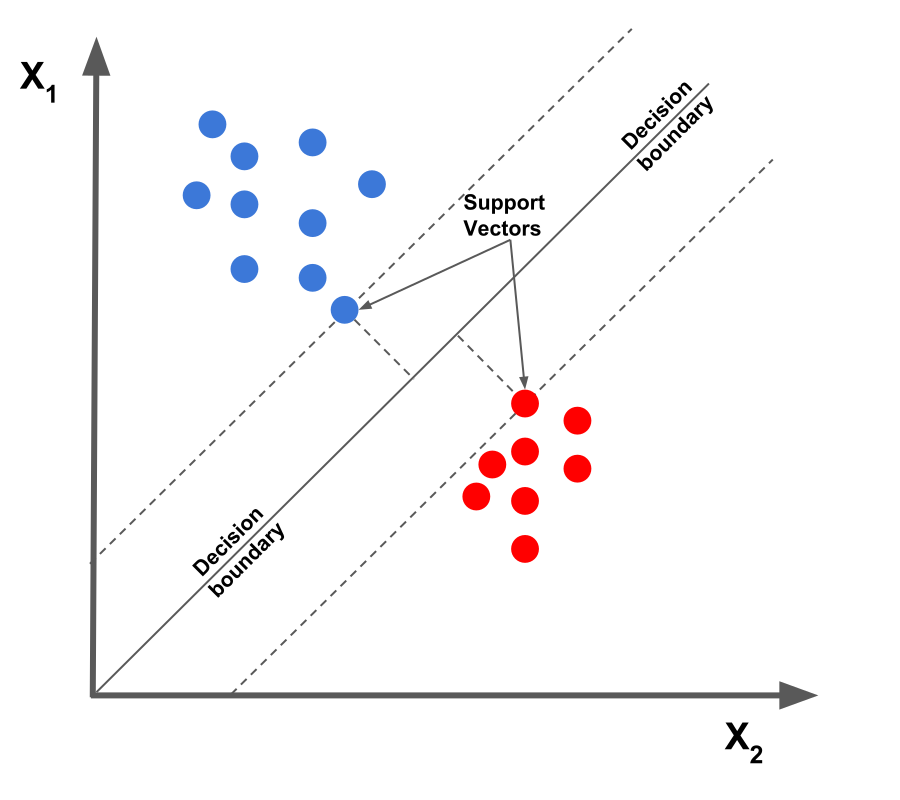
\includegraphics[width=0.5\linewidth]{imgs/svm}}
\end{figure}

\subsection{Hard-margin SVM}

Предположим что наша выборка линейно разделима. Тогда искомая гиперплоскость:

\begin{equation}
	\bm{x}^T\beta - \beta_0 = 0; \beta \in  \mathbb{R}^{p}, \beta_0 \in \mathbb{R}
	\label{16}
\end{equation}

А классифицирующие правило строится следующим образом:

\begin{equation}
	\begin{split}
	 g(x) =  \bm{x}^T \beta - \beta_0, \\
	 \bm{\Phi}(x) =  sign ( g(x) ).
	\end{split}
	\label{17}
\end{equation}

Уравнения пары гиперплоскостей с точностью до нормировки:

\begin{equation}
	\begin{split}
		\bm{x}^T \beta - \beta_0 = -1, \\
		\bm{x}^T \beta - \beta_0 = 1.
	\end{split}
	\label{18}
\end{equation}

А расстояние между ними равно: $\dfrac{2}{||\beta||}$

Принадлежность точек обучающей выборки описывается как отступ (\ref{19}) от разделяющей гипер плоскости. Отступ всегда больше или равен $1$, так как наша выборка линейно разделима.

\begin{equation}
	M_i = (\bm{x}^T \beta - \beta_0)y_i \geqslant 1
	\label{19}
\end{equation}

Задача построения разделяющей гиперплоскости сводится к задаче квадратичного программирования с линейными ограничениями:

\begin{equation}
	\begin{cases}
		\frac{1}{2}||\beta||_2^2\rightarrow \min\limits_{\beta,\beta_0} \\
		M_i  \geqslant 1 \\
	\end{cases}
	\label{20}
\end{equation}

\subsection{Soft-margin SVM}

Передем к случаю когда выборка линейно не разделима, тогда задача \ref{20} не имеет решения, так как система неравенств несовместна. Перепишем задачу \ref{20}, добавим небольшие изменения.

\begin{equation}
	\begin{cases}
		\frac{1}{2}||\beta||_2^2 + C \sum \xi_i \rightarrow \min\limits_{\beta,\beta_0, \xi} \\
		M_i \geqslant 1 - \xi_i \\
		\xi_i \geqslant 0 \\
	\end{cases}
	\label{21}
\end{equation}

Теперь мы разрешили объектам нарушать границы разделяющей гиперплоскости. Так же мы добавили сумму этих нарушений $\xi$ с весом $C$ в минимизируемый функцианал, чтобы подобрать такую гиперплоскость в которой объектов <<нарушителей>> будет наименьшим.

Применим условия Каруши-Куна-Таккера к задаче \ref{21}. Запишем функцию Лагранжа:

\begin{equation}
	L(\beta, \beta_0, \xi; \lambda, \eta) =  \frac{1}{2} ||\beta||^2 - \sum\limits_{i=1}^{n}(M_i - 1) - \sum\limits_{i=1}^{n} \xi_i(\lambda_i + \eta_i - C)
	\label{22}
\end{equation}

$\lambda_i$ --- переменные, двойственные к ограничениям $M_i \geqslant 1 - \xi_i$,

$\eta_i$ --- переменные, двойственные к ограничениям $\xi_i \geqslant 0 $.\\


Также запишем условия для первых производных функции Лагранжа, исходные ограничения, ограничения к двойственным переменным и условиями дополняющей нежесткости.

\begin{equation}
	\begin{cases}
		\dfrac{\partial L}{\partial \beta} = 0, \dfrac{\partial L}{\partial \beta_0} = 0, \dfrac{\partial L}{\partial \xi} = 0; \\
		\xi_i \geqslant 0, \lambda_i \geqslant 0, \eta_i \geqslant 0, i = 1, \dotsc, n; \\
		\lambda_i = 0 \text{ либо } M_i = 1 - \xi_i, i = 1, \dotsc, n; \\
		\eta_i = 0 \text{ либо } \xi_i = 0, i = 1, \dotsc, n;
	\end{cases}
	\label{23}
\end{equation}

Распишем производные поподробнее, получаем необходимые условия седловой точки функции Лагранжа:
\begin{equation}
	\begin{split}
 	\dfrac{\partial L}{\partial \beta} = \beta - \sum\limits_{i=1}^{n}\lambda_i y_i \bm{x}_i = 0 \Longrightarrow \beta = \sum\limits_{i=1}^{n}\lambda_i y_i \bm{x}_i \\
 	\dfrac{\partial L}{\partial \beta_0} = - \sum\limits_{i=1}^{n}\lambda_i y_i = 0 \Longrightarrow \sum\limits_{i=1}^{n}\lambda_i y_i = 0 \\
 	\dfrac{\partial L}{\partial \xi_i} = \lambda_i - \eta_i - C = 0 \Longrightarrow \lambda_i + \eta_i = C, i = 1, \dotsc, n; 
 	\end{split}
 	\label{24}
\end{equation}

Из этих условий можем записать типизацию объектов:

\begin{enumerate}
	\item $ \lambda_i = 0; \eta_i = C; \xi = 0; M_i \geqslant 1 $ - неинформативные объекты.
	\item $ 0 < \lambda_i < C; 0 < \eta_i < C; \xi = 0; M_i = 1 $ - опорные граничные объекты.
	\item $ \lambda_i = C; \eta_i = 0; \xi > 0; M_i < 1 $ - опорные-нарушители.
\end{enumerate}

Из формул \ref{24} видно, что объекты отступ $M_i$ которых больше $1$ не участвуют в построении разделяющей гиперплоскости. 

Отсюда можно дать определение опорным объектам. Объект $x_i$ называется опорным, если $\lambda_i \neq 0$.

Избавимся от всех переменных, кроме двойственных в \ref{22}, получим:

\begin{equation}
	\begin{cases}
		-L(\bm{\lambda}) = - \sum\limits_{i=1}^n \lambda_i + \frac{1}{2} \sum\limits_{i=1}^{n}\sum\limits_{j=1}^{n} \lambda_i \lambda_j y_i y_j (x_i, x_j) \rightarrow \min\limits_{\bm{\lambda}}; \\
		0 \leqslant \lambda_i \leqslant C, i = 1, \dotsc, n; \\
		\sum\limits_{i=1}^{n} \lambda_i y_i = 0.
	\end{cases}
	\label{25}
\end{equation}

Решение прямой задачи выражается через решение двойственной:

\begin{equation}
	\begin{cases}
		\beta = \sum\limits_{i=1}^n \lambda_i y_i x_i;\\
		\beta_0 = \langle\beta, \bm{x}_i\rangle - y_i, \text{ для любого } i: \lambda_i > 0, M_i = 1.
	\end{cases}
	\label{26}
\end{equation}

Тогда 

Линейный классификатор с признаками $f_i(x) = \langle x, x^{'} \rangle $: 
\begin{equation} 
	\bm{\Phi}(x) = sign ( \sum\limits_{i=1}^{n} \lambda_i y_i \langle\bm{x}, \bm{x}_i\rangle - \beta_0) 
	\label{27}
\end{equation}

\subsection{Минимизация эмпирического риска}

Как и в случае задачи минимизации \ref{11} (логистической регрессии), можем записать задачу минимизации в общей форме:

\begin{equation*} 
Q(\beta) = \sum\limits_{i = 1}^{n} \hat{\mathfrak{L}}( M_i )  \rightarrow \min\limits_{\beta}
\end{equation*}

Чтобы получить SVM достаточно взять $\hat{\mathfrak{L}}(M) = \max(0, 1 - M)$. В случае SVM $M_i = g(x_i, \beta)y_i = (\bm{x}_i^T \beta - \beta_0)y_i$.

Подставляя функцию потерь и отступ, получаем задачу минимизации:

\begin{equation} 
	Q(\beta) = \sum\limits_{i = 1}^{n} \max(0, 1 - (\bm{x}_i^T \beta - \beta_0)y_i)  \rightarrow \min\limits_{\beta}
	\label{27}
\end{equation}

\subsection{Нелинейное обобщение}
	Можно заменить $ \langle x, x^{'} \rangle $ в \ref{27} на нелинейную функцию $K( x, x^{'} )$. \\

	Определение: Функция $K: X \times X \rightarrow \mathbb{R}$ --- ядро, если $K(\bm{x}, \bm{x}^{'}) = \langle \phi(\bm{x}), \phi(\bm{x}^{'}) \rangle$ при некотором $\phi: X \rightarrow H$, где $H$ --- гильбертово пространство.
	
	Данное соображение позволяет применять SVM к данным в достаточной степени линейно разделимым в некотором гильбертовом пространстве (в том числе --- бесконечномерном); в том числе --- без предъявления в явном виде отображения из исходного пространства в данное.
	
	\begin{figure}[h]
		\centering
		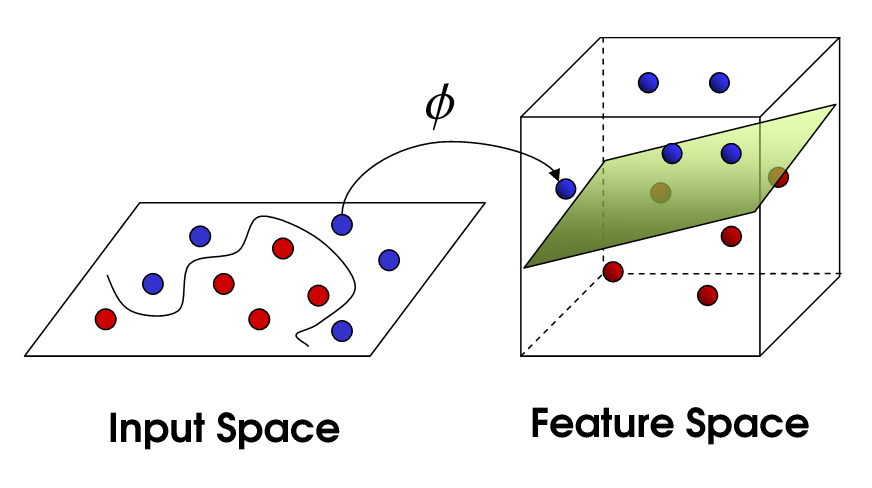
\includegraphics[width=0.7\linewidth]{imgs/kernels}
	\end{figure}

	Так как непосредственная проверка положительной определённости ядра представляет собой проблему, можно воспользоваться следующими операциями, приводящими к получению новых ядер:
	
	\begin{itemize}
		\item Скалярное произведение в векторном пространстве
		\item Положительная константа
		\item Произведение ядер: $K(u, v) = K_1(u, v) K_2(u, v)$
		\item Произведение отображений: $K(u, v) = \phi(u)\phi(v), \phi: x \rightarrow \mathbb{R}$
		\item Линейная комбинация с положительными коэффициентами: $K(u, v) = \alpha_1 K_1(u, v) + \alpha_2 K_2(u, v), \alpha_{1,2} > 0$
		\item Композиция ядра и отображения: $K(u, v) =  K_1(\phi(u), \phi(v))$
		\item Степенной ряд: $$ f: \mathbb{R} \rightarrow \mathbb{R}$$ сходящийся степенной ряд с положительными коэффициентами, тогда $$ K(u, v) = f(K_1(u, v)) $$ является ядром.
	\end{itemize} 
	
	
	Часто используемые ядра:
	\begin{itemize}
		\item RBF (radial basis functions): $K(x, x^{'}) = e^{-\gamma ||x - x^{'}||_2^2}$
		\item Полиномиальное (степеней $\leqslant d : K(x, x^{'}) = (\langle x - x^{'} \rangle + 1)^d$)
	\end{itemize} 


\section{Кросс-валидация}
Кросс-валидация (перекрестная проверка, скользящий контроль) --- процедура эмпирического оценивания обобщающей способности алгоритмов. С помощью кросс-валидации "эмулируется" наличие тестовой выборки, которая не участвует в обучении модели, но для которой известны правильные ответы. Среди видов перекрестной проверки встречаются следующие:
\begin{itemize}
	\item Валидация на отложенных данных (Hold-Out Validation);
	\item Полная кросс-валидация (Complete Cross-Validation);
	\item k-fold Cross-Validation;
	\item t$\times$k-fold Cross Validation;
	\item Кросс-валидация по отдельным объектам (Leave-One-Out);
	\item Случайные разбиения (Random Subsampling).
\end{itemize}

\subsection{Кросс-валидация: Hold-Out Validation}

Обучающая выборка один раз случайным образом разбивается на две части $\bm{T} = \bm{T}^t \cup \bm{T}^{N-t}$.


\begin{figure}[h]
	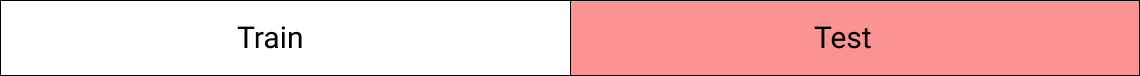
\includegraphics[width=0.9\linewidth]{imgs/hold-out}
\end{figure}

После чего решается задача оптимизации:
$$ HO(\mu, \bm{T}^t, \bm{T}^{N-t}) = \mathfrak{L}(\mu(\bm{T}^t), \bm{T}^{N-t}) \rightarrow min $$.


Метод Hold-out применяется в случаях больших датасетов, т.к. требует меньше вычислительных мощностей по сравнению с другими методами кросс-валидации. 

Недостатком метода является то, что оценка существенно зависит от разбиения, тогда как желательно, чтобы она характеризовала только алгоритм обучения.

\subsection{Кросс-валидация: Complite cross-validatio}

\begin{itemize}
	\item Выбирается значение $t$;
	\item Выборка разбивается всевозможными способами на две части $\bm{T} = \bm{T}^t \cup \bm{T}^{N-t}$.
\end{itemize}
\begin{figure}[h]
	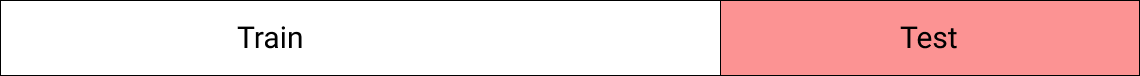
\includegraphics[width=1\linewidth]{imgs/completecrossvalidation}
\end{figure}
После чего решается задача оптимизации:
$$ CVV_t = \frac{1}{C_N^{N-t}}\sum\limits_{\bm{T}^N = \bm{T}^t \cup \bm{T}^{N-t}} \mathfrak{L}(\mu(\bm{T}^t), \bm{T}^{N-t}) \rightarrow min $$.


Здесь число разбиений $ C_N^{N-t} $ становится слишком большим даже при сравнительно малых значениях $ t $, что затрудняет практическое применение данного метода.


\subsection{Кросс-валидация: k-fold Cross-Validation}
\begin{itemize}
	\item $\bm{T}^l$ разбивается на $ \bm{T_1}\cup\cdots\cup\bm{T_k}, |\bm{T_i}|\approx \frac{1}{k} $ частей;
	\item Производится $ k $ итераций:
	\begin{itemize}
		\item Модель обучается на $ k-1 $ части обучающей выборки;
		\item Модель тестируется на части обучающей выборки, которая не участвовала в обучении.
	\end{itemize}
\end{itemize}
Каждая из $ k $ частей единожды используется для тестирования.

\begin{figure}[h]
	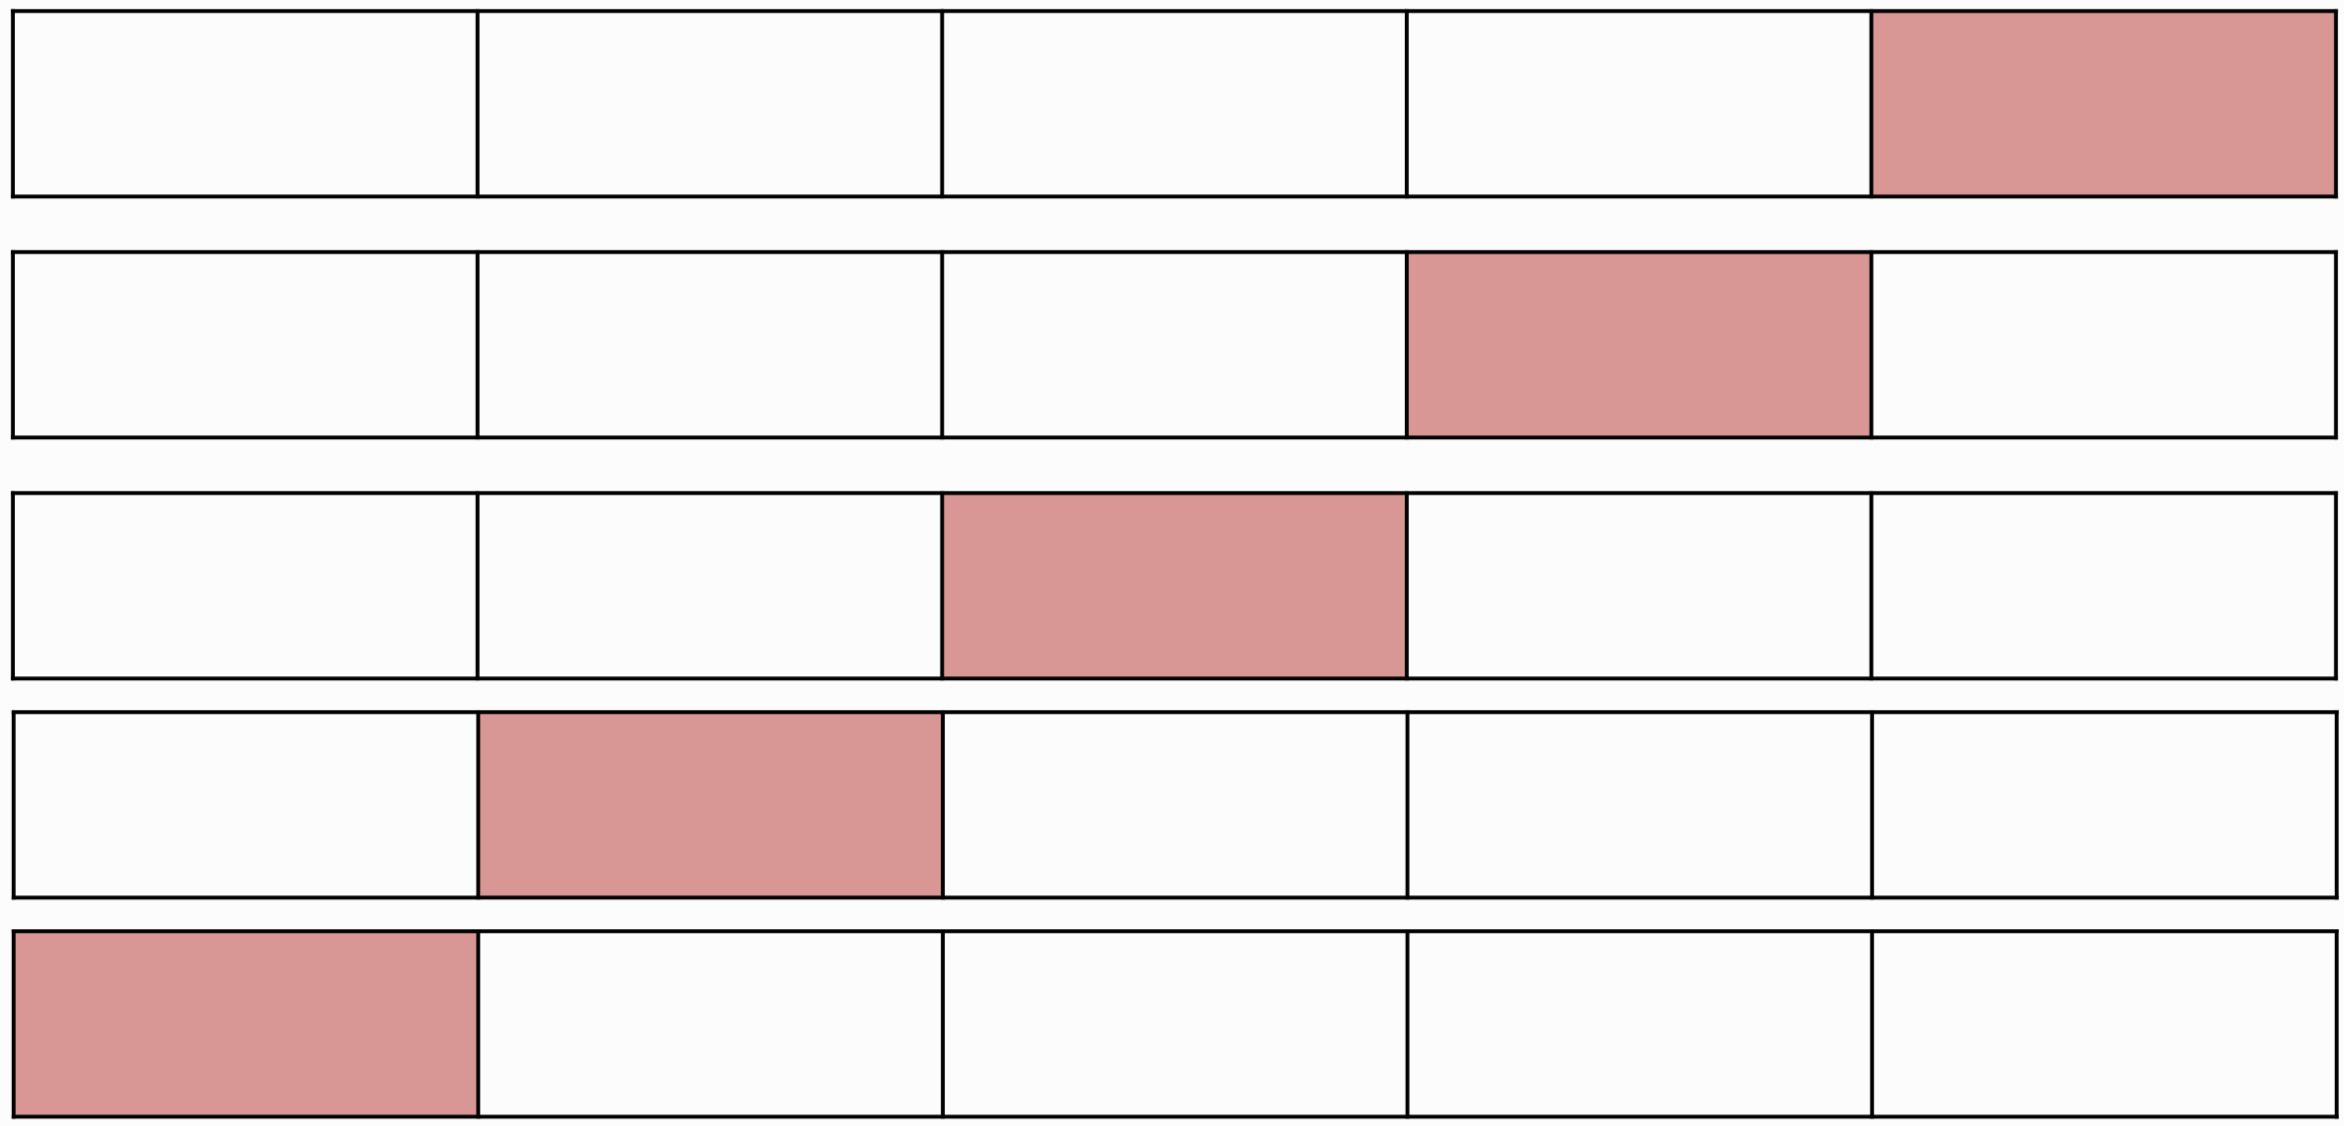
\includegraphics[width=1\linewidth]{imgs/K-fold-validation}
\end{figure}
После чего решается задача оптимизации:
$$ CV_k = \frac{1}{k}\sum\limits_{i=1}^k\mathfrak{L}(\mu(\bm{T}^N \setminus \bm{T}_i), \bm{T}_i) \rightarrow min $$.


\subsection{Кросс-валидация: t$\times$k-fold Cross Validation}
\begin{center}
	\textit{Как k-fold Cross-Validation, только $t$ раз.}
\end{center}

Разбиение:
$\bm{T}^N = \bm{T}_{(1,1)}\cup\cdots\cup\bm{T}_{(k,1)}=\bm{T}_{(1,t)}\cup\cdots\cup\bm{T}_{(k,t)},|\bm{T}_{(i,j)}|\approx \frac{N}{k} $, 

Задача оптимизации: 
$$ CV_{t\times k} = \frac{1}{tk}\sum\limits_{j=1}^t\sum\limits_{i=1}^k\mathfrak{L}(\mu(\bm{T}^N \setminus \bm{T}_{(i,j)}), \bm{T}_{(i,j)}) \rightarrow min $$


\subsection{Кросс-валидация: Leave-One-Out}

Выборка разбивается на $ N-1 $ и $ 1 $ объект $ N $ раз.
$LOO = \frac{1}{N}\sum\limits_{i=1}^N\mathfrak{L}(\mu(\bm{T}^N \setminus p_i), p_i) \rightarrow min$, где $ p_i = (x_i, y_i) $.

Преимущества LOO в том, что каждый объект ровно один раз участвует в контроле, а длина обучающих подвыборок лишь на единицу меньше длины полной выборки.

Недостатком LOO является большая ресурсоёмкость, так как обучаться приходится $ N $ раз.

\subsection{Кросс-валидация: Random subsampling (Monte-Carlo cross-validation)}
Выборка разбивается в случайной пропорции. Процедура повторяется несколько раз.

\begin{figure}[h]
	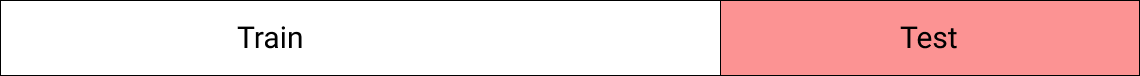
\includegraphics[width=1\linewidth]{imgs/completecrossvalidation}
\end{figure}

\subsection{Кросс-валидация: Выбор лучшей модели}
Обычно, с помощью кросс-валидации находят лучшие параметры модели в рассматриваемой задаче. Весь набор данных делят на тренировочную и тестовую выборки, после чего эмпирически находят лучшие параметры средством перекрестной проверки на тренировочном наборе и оценивают эффективность модели на тестовом множестве.

\begin{figure}[h]
	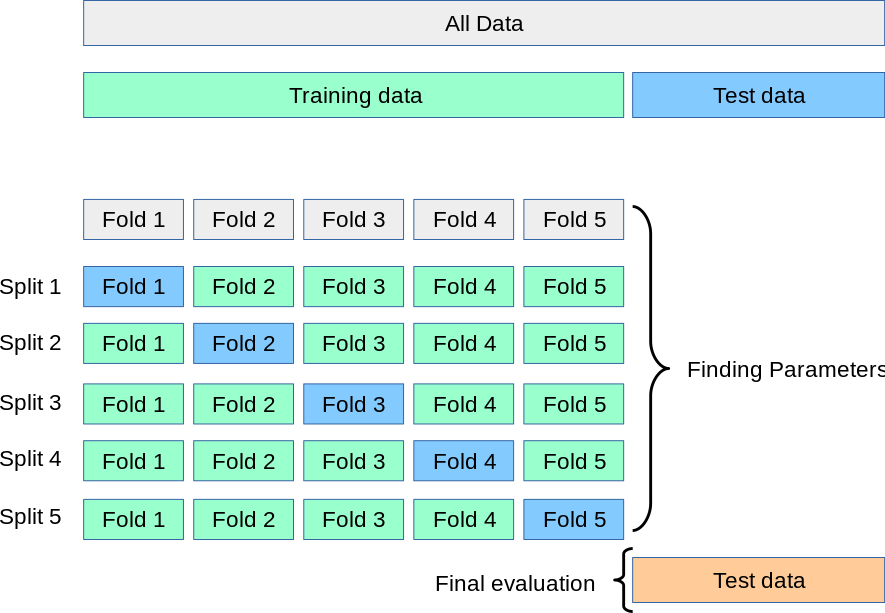
\includegraphics[width=1\linewidth]{imgs/model_selection}
\end{figure}

Исходя из полученных результатов принимается окончательное решение - искать другие параметры или остановиться на текущей модели и ее конфигурации.

\section{SGD}
Стохастический градиентный спуск - оптимизационный алгоритм, при котором градиент оптимизируемой функции считается на каждой итерации от случайно выбранного элемента выборки.

Введем дополнительные обозначения:
\begin{itemize}
	\item $ \bm{X}^l $ --- обучающая выборка, состоящая из пар $ (x_i, y_i)_{i=1}^l $;
	\item $ a(x, \omega) $ --- семейство алгоритмов с параметром вектора весов $ \omega $;
\end{itemize}


Так как стохастический градиентный спуск является модификацией всеми известного градиентного спуска, начнем с последнего.

Найдем алгоритм $ a(x, \omega) $, аппроксимирующий зависимость $ y^* $.

Например, в случае линейного классификатора искомый алгоритм имеет вид:
$$ a(x, \omega) = \phi(\sum\limits_{j=1}^N \omega_jx^j - \omega_0), $$где $ \phi(z) $ - функция активации. 

\textit{Решаемая задача оптимизации:}
$$ Q(\omega) = \frac{1}{N}\sum\limits_{i=1}^{N}\mathfrak{L}(a(x_i, \omega), y_i)\rightarrow\min\limits_{\omega} $$
\textit{Обновление весов:}
$$ \omega^{(t+1)} = \omega^{(t)} - h\nabla Q(\omega^{(t)}) $$

Проблема GD --- чтобы определить новое приближение вектора весов необходимо вычислить градиент от каждого элемента выборки, что может сильно замедлять алгоритм.
Идея ускорения заключается в использовании либо одного элемента (SGD), либо некоторой подвыборки (Batch GD) для получения нового приближения весов. 

\textit{Веса, при подходе SGD, обновляются следующим образом:}

$$ \omega^{(t+1)} = \omega^{(t)} - h\nabla\mathfrak{L}(a(x_i, \omega^{(t)}), y_i),$$ где $ i $ --- случайно выбранный индекс.

Т.к. направление изменения $ \omega $ будет определяться за $ O(1) $, подсчет $ Q $ на каждом шаге будет слишком дорогостоящим. Для ускорения оценки, будем использовать одну из рекуррентных формул:
\begin{itemize}
	\item Среднее арифметическое: $ \overline Q_m = \frac{1}{m}\mathfrak{L}(a(x_{i_m}, \omega^{(m)}), y_{i_m}) + (1 - \frac{1}{m}) \overline Q_{m-1}$;
	\item Экспоненциальное скользящее среднее: $ \overline Q_m = \lambda\mathfrak{L}(a(x_{i_m}, \omega^{(m)}), y_{i_m}) + (1 - \lambda) \overline Q_{m-1}$, где $ \lambda $ --- темп забывания "предыстории" ряда.
\end{itemize}

Так как алгоритм итеративный, нужно задать начальные значения весов оптимизируемой модели. Существует несколько способов инициализации весов, например:

\begin{itemize}
	\item $ \omega_0 = 0 $;
	\item $ \omega_0 = random(-\frac{1}{2n}, \frac{1}{2n}) $;
\end{itemize}

Говоря о сходимости, установлено, что если скорость обучения убывает при увеличении числа итераций SGD сходится почти наверняка к глобальному минимуму в случае выпуклой или псевдовыпуклой функции $ Q(\omega) $, в противном случае метод сходится почти наверняка к локальному минимуму.


Достоинства:
\begin{itemize}
	\item Легко реализуется;
	\item Функция потерь и семейство алгоритмов могут быть любыми (если функция потерь не дифференцируема, ее можно аппроксимировать дифференцируемой);
	\item Легко добавить регуляризацию;
	\item Возможно потоковое обучение;
	\item Подходит для задач с большими данными, иногда можно получить решение даже не обработав всю выборку.
\end{itemize}

Недостатки:
\begin{itemize}
	\item Нет универсального набора эвристик, их нужно выбирать для конкретной задачи отдельно;
	\item На практике остаются проблемы с локальными экстремумами.
\end{itemize}

Модификации:
\begin{itemize}
	\item Не выраженные явно изменения (ISGD) --- градиент пересчитывается на следующей итерации;
	\item Метод импульса --- запоминает $ \Delta\omega $ на каждой итерации и определяет следующее изменение в виде линейной комбинации градиента и предыдущего изменения;
	\item Усреднённый стохастический градиентный спуск;
	\item AdaGrad --- модификация SGD с отдельной для каждого параметра скоростью обучения;
	\item RMSProp --- это метод, в котором скорость обучения настраивается для каждого параметра. Идея заключается в делении скорости обучения для весов на скользящие средние значения недавних градиентов для этого веса;
	\item Adam --- это обновление оптимизатора RMSProp. Здесь используются скользящие средние как градиентов, так и вторых моментов градиентов.
\end{itemize}















	
\end{document}